\section{ERF Error Function}

\subsection{Usage}

Computes the error function for real arguments.  The \verb|erf|
function takes only a single argument
\begin{verbatim}
  y = erf(x)
\end{verbatim}
where \verb|x| is either a \verb|float| or \verb|double| array.  The output
vector \verb|y| is the same size (and type) as \verb|x|.
\subsection{Function Internals}

The erf function is defined by the integral:
\[
  \mathrm{erf}(x) = \frac{2}{\sqrt{\pi}}\int_{0}^{x} e^{-t^2} \, dt,
\]
and is the integral of the normal distribution.
\subsection{Example}

Here is a plot of the erf function over the range \verb|[-5,5]|.
@>
which results in the following plot.


\centerline{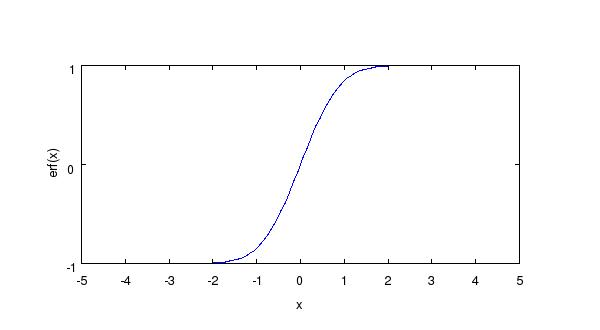
\includegraphics[width=8cm]{erf1}}

